\section{Simple Aircraft Design}

We finally implemented our RSP heuristic algorithm on a simple aircraft design problem. 
In this problem, we conduct an aerostructural optimization of a wing and fuselage given a payload and a range requirement. 

% We implemented the RSP formulation ideas above on a simple aircraft design problem, with 12 uncertain variables,
% and a single signomial constraint. . A short overview of the model follows.

\subsection{Model Description}

Below we briefly describe the different sub-models of our simple aircraft design, and then specify the different uncertainties in this model.

\subsubsection{Lift, Weight, Drag and Thrust}
This aircraft is assumed to be in a steady, level flight. 
Accordingly, we can assume that the thrust generated by the aircraft is equal to the drag,
and the lift generated by the wing is equal to the total weight.

Both the wing and the fuselage contribute to the total drag in our model.
The wing drag is divided into induced and profile drag, while the fuselage drag is proportional to the fuel volume in the fuselage.
Note that the model does not assume limitations on thrust, but instead assumes constant thrust specific fuel consumption. Moreover, the model assumes constant airfoil thickness to chord ratio.

The weight of the aircraft is the sum of the payload weight, wing weight, and
the fuselage weight, as shown in Figure~\ref{fig:liftweight}. Lift is generated by the wing,
which is described by an aspect ratio $A$ and surface area $S$.

\begin{figure}[ht]
\centering
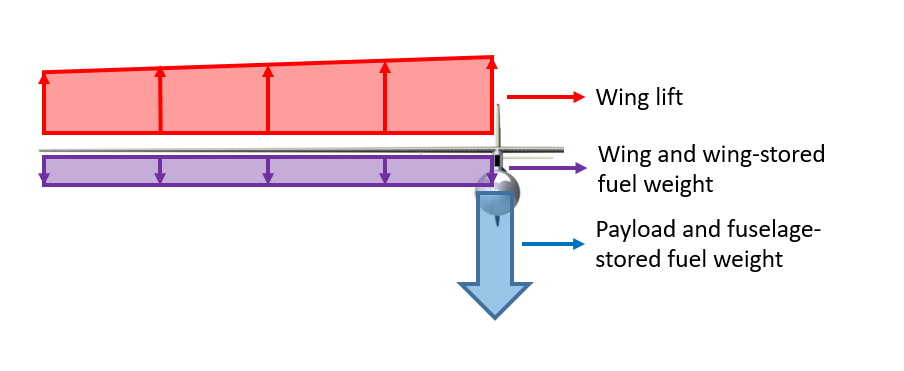
\includegraphics[width=0.8\textwidth]{liftweight.PNG}
\caption{\label{fig:liftweight} Wing lift is equal and opposite to the wing weight, payload weight, and total fuel weight.}
\end{figure}

\subsubsection{Wing Structure}
The wing structure model is based on a simple beam model with a distributed lift load,
and a point mass in the center representing the fuselage, as shown in Figure~\ref{fig:liftweight}.

\subsubsection{Fuel Volume}
The fuel in the aircraft can be stored either in the wing or in the fuselage.
The signomial constraint in the optimization appears in the fuel volume model as in Equation~\ref{eq:fuel}:

\begin{equation}
\label{eq:fuel}
V_f \leq V_{f_{wing}} + V_{f_{fuse}} 
\end{equation}

where $V_{f_{wing}}$ and $V_{f_{fuse}}$ represent the fuel volume available in the wing
and the fuselage respectively. They are each represented by the following monomial constraints.

\begin{equation}
\label{eq:fuelwing}
V_{f_{wing}} <= 3e^{-2}\frac{S^{1.5}\tau}{A^{0.5}}
\end{equation}

\begin{equation}
\label{eq:fuelfuse}
V_{f_{fuse}} <= 10 \times CDA_0
\end{equation}

Where $S$ is the total wing area, $\tau$ is the airfoil thickness ratio, $A$ is the wing aspect ratio, and $CDA_0$ is the fuselage drag area. 
Note that the monomials above are represented with inequalities, to be compatible with the RSP formulation.

\subsubsection{Takeoff constraints}
We specify that the aircraft has to be able to takeoff at a speed of $V_{min}$
without exceeding the aircraft stall lift coefficient $C_{L_{max}}$, both of which are
specified with an associated uncertainty.

\subsubsection{Uncertainties}

The uncertainties for the different constants in the problem have been determined
considering the parameters in aircraft design that often have the largest uncertainty.
These uncertainties are listed in Table~\ref{tab:uncertainties}.

\begin{center}
\begin{tabular}{ |m{11em}|m{5cm}|m{5cm}|}
\hline
Uncertain Parameter & Value & Description \\
\hline
$S_{wetratio}$ & $2.075 \pm 3\%$ & wetted area ratio\\
\hline
$e$ & $0.920 \pm 3\%$ & span efficiency \\
\hline
$\mu$ & $1.775e^{-5}$ $[kg/(ms)]$ $\pm 4\%$ & viscosity of air\\
\hline
$\rho$ & $1.230$ $[kg/m^3]$ $\pm 5\%$  & air density\\  
\hline
$C_{L_{max}}$ & $1.600 \pm 5\%$ & stall lift coefficient\\
\hline
$k$ & $1.170 \pm 10\%$ & fuselage form factor\\
\hline
$\tau$ & $0.120 \pm 10\%$ & airfoil thickness ratio\\
\hline
$N_{ult}$ & $3.300 \pm 15\%$ & ultimate load factor\\
\hline
$V_{min}$ & $25.00$ $[m/s]$ $\pm 20\%$ & takeoff speed\\
\hline
$W_0$ & $6250$ $[N]$ $\pm 20\%$ & payload weight\\
\hline
$W_{w_{coeff1}}$ & $2.000e^{-5} $ $[\frac{1}{m}]$ $\pm 20\%$ & Wing Weight Coefficient 1\\
\hline
$W_{w_{coeff2}}$ & $60.00 $ $[Pa]$ $\pm 20\%$ & Wing Weight Coefficient 2\\  
\hline
\end{tabular}
\captionof{table}{Uncertain parameters in the signomial simple aircraft design.}
\label{tab:uncertainties}
\end{center}

The parameter uncertainties reflect aerospace engineering intuition.
The wing weight coefficients $W_{w_{coeff1}}$ and $W_{w_{coeff2}}$, and the ultimate load factor $N_{ult}$ have
large uncertainty because the build quality of aircraft components is often difficult to quantify with a large degree of certainty.
The payload weight ($W_0$) has a large uncertainty, because it is valuable if the aircraft
has the flexibility to accommodate larger payloads. Parameters that engineers take to be
physical constants ($\mu$, $\rho$) and those that can be determined/manufactured with a relatively
high degree of accuracy ($S_{wetratio}$, $e$) have relatively low deviations.
Parameters that require testing to determine ($C_{L_{max}}$, $V_{min}$) have a level of uncertainty
that reflects the expected variance of the parameters.

\subsection{Optimization Results}

The problem is optimized for different sizes of box and elliptical uncertainty sets by varying the parameter $\Gamma$ as defined in Appendix \ref{LP_to_GP}. The design variables are then fixed for each solution so that the design can be simulated for 1000 different realizations of the uncertain parameters in table \ref{tab:uncertainties} to examine average design performance.\\

\begin{figure}[ht]
    \centering
    \captionsetup{justification=centering, font=small}
    \begin{subfigure}{0.49\textwidth}
        \centering
        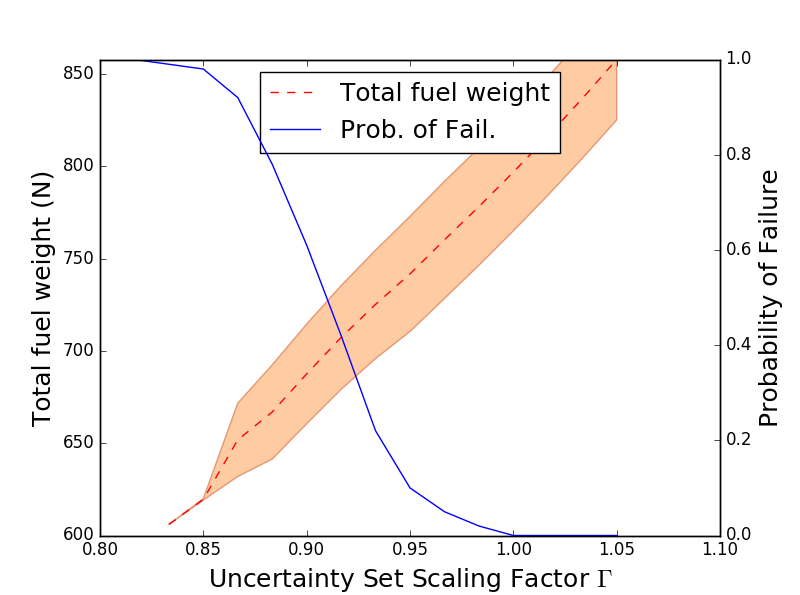
\includegraphics[height=2.3in]{signomial_simple_flight/box_best_pairs.png}
        % \caption{Box Uncertainty Set Objective Value}
    \end{subfigure}%
    ~ 
    \begin{subfigure}{0.49\textwidth}
        \centering
        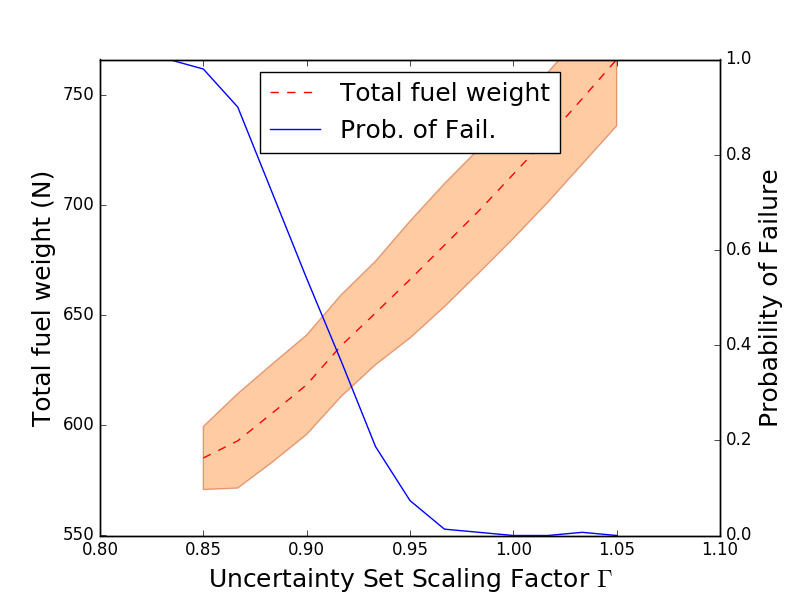
\includegraphics[height=2.3in]{signomial_simple_flight/ell_best_pairs.png}
        % \caption{Box Uncertainty Set Probability of Failure}
    \end{subfigure}
    \caption{Performance of the optimal robust signomial simple aircraft, using the Best Pairs formulation, as a function of $\Gamma$ for different uncertainty sets.}
    \label{signomial_var_gamma}
\end{figure}

We can see from Figure \ref{signomial_var_gamma} that probability of failure goes to zero as $\Gamma$ increases. 
Obviously, it is worth using elliptical uncertainty sets for this aircraft design problem as the performance is significantly better than that of a box uncertainty set, despite the increase in complexity. 
Moreover, using margins would in the best case be as good as using a box uncertaintyset, and therefore will lead to an inferior performance.

Figure \ref{compare_signomial} compares the different methodologies in terms of run times, number of constraints, and average performance. The Best Pairs and Linearized Perturbations achieves good performance, however the Best Pairs methodology needs the most number of constraints, while the Linearized perturbations requires the most setup and solve time. The Simple Conservative formulation is significantly faster than the other formulations and requires the least number of additional constraints.
\ \\
\ \\

\begin{figure}[ht]
    \centering
    \captionsetup{justification=centering, font=small}
    \begin{subfigure}{0.499\textwidth}
        \centering
        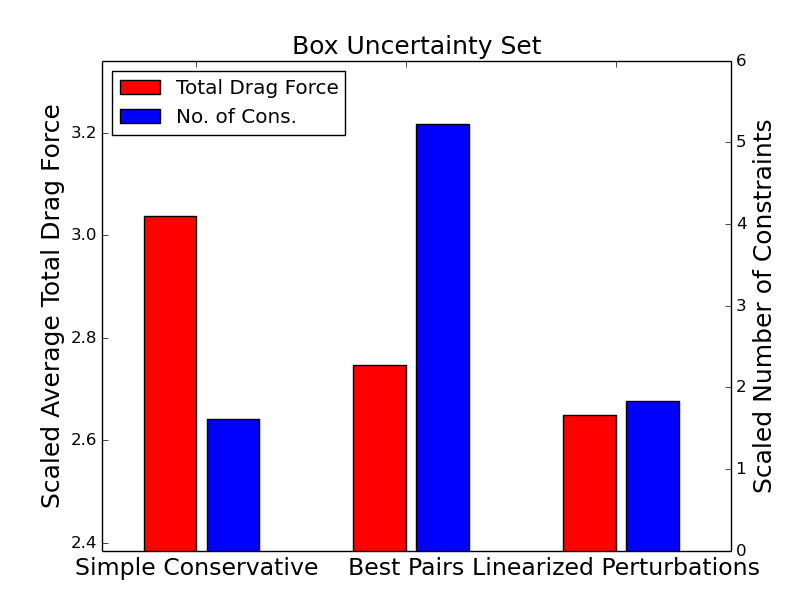
\includegraphics[height=2.3in]{signomial_simple_flight/box.png}
        % \caption{Box Uncertainty Set Objective Value}
    \end{subfigure}%
    ~ 
    \begin{subfigure}{0.49\textwidth}
        \centering
        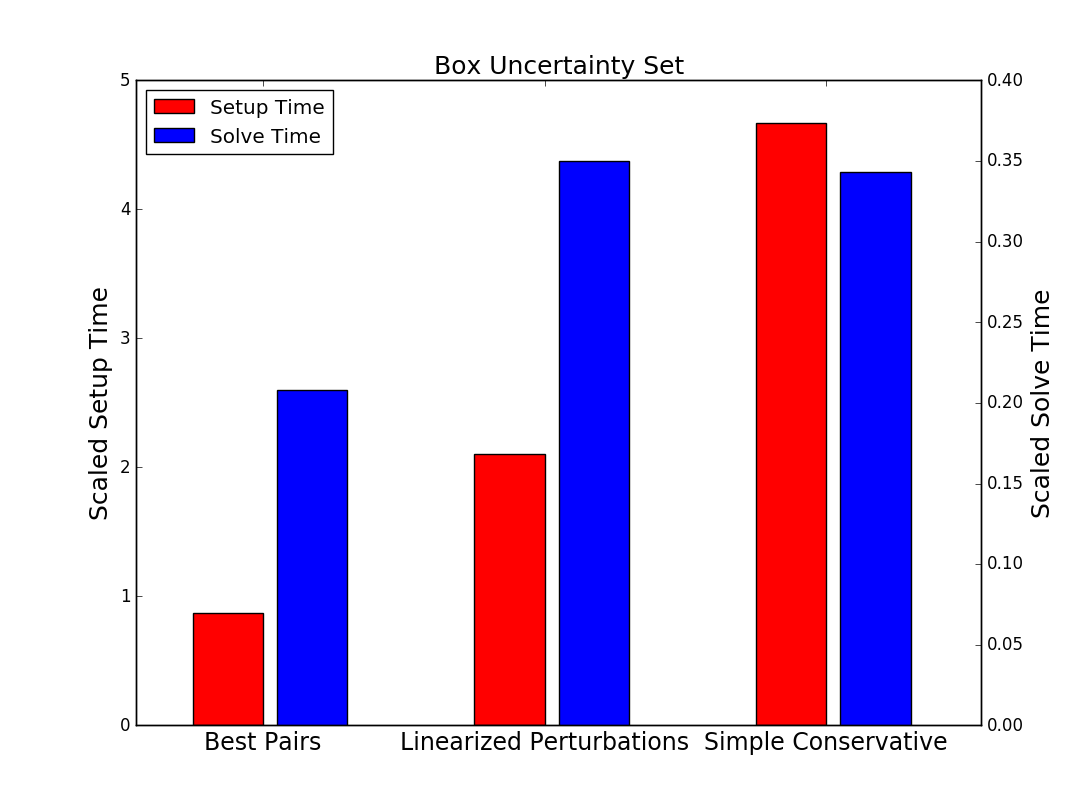
\includegraphics[height=2.3in]{signomial_simple_flight/box_times.png}
        % \caption{Box Uncertainty Set Probability of Failure}
    \end{subfigure}
    ~
    \begin{subfigure}{0.499\textwidth}
        \centering
        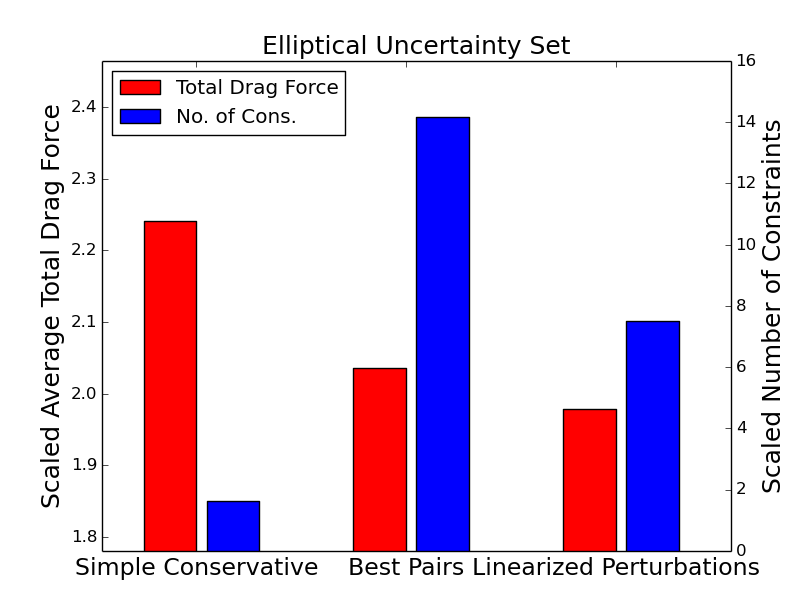
\includegraphics[height=2.3in]{signomial_simple_flight/ell.png}
        % \caption{Elliptical Uncertainty Set Objective Value}
    \end{subfigure}%
    ~ 
    \begin{subfigure}{0.49\textwidth}
        \centering
        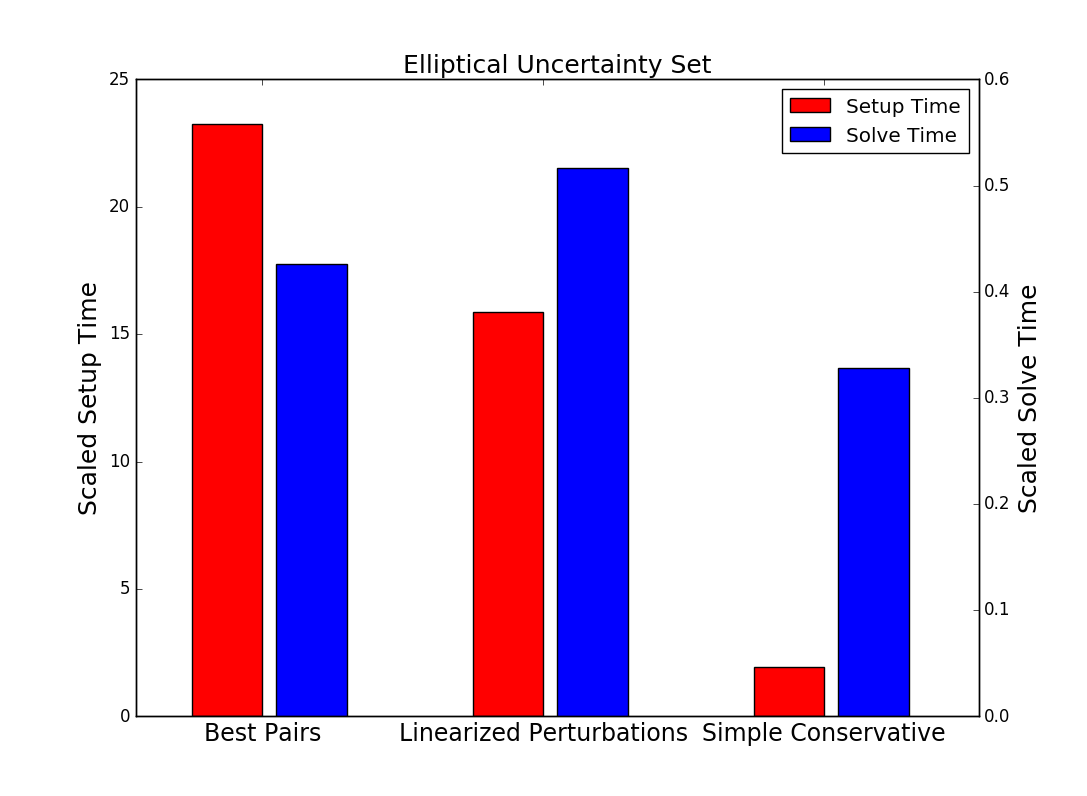
\includegraphics[height=2.3in]{signomial_simple_flight/ell_times.png}
        % \caption{Elliptical Uncertainty Set Probability of Failure}
    \end{subfigure}
    \caption{Robust signomial simple aircraft design results relative to the deterministic design problem.}
    \label{compare_signomial}
\end{figure}

\subsection{The Effect of Robustness}

\begin{figure}
\begin{center}
\begin{tikzpicture}[scale=0.5]
\tkzKiviatDiagram{$\frac{W_f}{L/D}$,$D$,$W_f$}
%solve for {W_f}{L/D}
\tkzKiviatLine[thick,
color=red,
mark=ball,
ball color=red,
mark size=3pt,opacity=.2,
fill=red!20](154.4/25,414.2/75,5180/700)
%solve for D
\tkzKiviatLine[thick,
color=blue,
mark=ball,
mark size=3pt,
fill=blue!20,
opacity=.5](161.8/25,400/75,5129/700)
% solve for {W_f}
\tkzKiviatLine[thick,
color=yellow,
mark=ball,
mark size=3pt,
fill= yellow!20,
opacity=.5](190.2/25,463.4/75,4536/700)
\end{tikzpicture}
\end{center}
\caption[Deterministic Spider Plot]{Design optimization of the aircraft with no uncertainty for 3 different objective functions.
The red, blue and yellow correspond to $\frac{W_f}{L/D}$, $D$, $W_f$ and objectives respectively.}
% tkz-kiviat documentation here in FRENCH: http://mirror.jmu.edu/pub/CTAN/macros/latex/contrib/tkz/tkz-kiviat/doc/TKZdoc-kiviat-main.pdf
\label{fig:spiderplotnoUncert}
\end{figure}

To further demonstrate the capabilities of robust SPs in aircraft design,
we performed the optimization of the aircraft with no uncertainty and ellipsoidal uncertainty ($\Gamma = 1$)
for two more objective functions, and plotted the results on spider plots.
Spider plots are useful because they allow engineers to find non-dominated solutions among the solutions
that lie on the Pareto frontier of potential objective functions. The objective functions chosen
for this analysis were fuel burn over lift-to-drag ratio ($\frac{W_f}{L/D}$), drag ($D$), and fuel burn ($W_f$).

In the spider plots in Figures \ref{fig:spiderplotnoUncert} and \ref{fig:spiderplotEllUncert},
none of the solutions are non-dominated for both the no uncertainty and ellipsoidal uncertainty cases.
In a GP, it is not possible that one of the solutions is non-dominated since the solutions are globally optimal.
But since there is no guarantee in optimality for SPs, it is possible to find non-dominated solutions if
the obtained solution is a local optimum.

In the case where there is no non-dominated solution such as this one,
we take the internal areas of the triangle formed by each optimization to be the figure of merit.
The smaller the area in the triangle, the higher the performance of the proposed solution.
In the no uncertainty case shown in Figure~\ref{fig:spiderplotnoUncert}, the red solution with the
objective of $\frac{W_f}{L/D}$ has the smallest internal area. In the ellipsoidal case shown in
Figure~\ref{fig:spiderplotEllUncert}, the blue solution with the objective of $D$ has the smallest internal area.

This is an interesting result, because the presence of an uncertainty set is
shown to affect the efficacy of different objective functions to obtain solutions
with the best overall performance. The differences between the objective functions
in the simple aircraft design problem are minute, because the different potential objectives
have a high degree of coupling. It is likely that, if the three objective functions didn't
have high degree of coupling, that the internal areas of the solution triangles may differ
more significantly.

\begin{figure}
\begin{center}
\begin{tikzpicture}[scale=0.5]
\tkzKiviatDiagram{$\frac{W_f}{L/D}$,$D$,$W_f$}
%solve for {W_f}{L/D}
\tkzKiviatLine[thick,
color=red,
mark=ball,
ball color=red,
mark size=3pt,opacity=.2,
fill=red!20](568.6/100,1051/150,13500/1500)
%solve for D
\tkzKiviatLine[thick,
color=blue,
mark=ball,
mark size=3pt,
fill=blue!20,
opacity=.5](587/100,1024/150,13100/1500)
% solve for {W_f}
\tkzKiviatLine[thick,
color=yellow,
mark=ball,
mark size=3pt,
fill= yellow!20,
opacity=.5](687.9/100,1155/150,11900/1500)
\end{tikzpicture}
\end{center}
\caption[Uncertain Spider Plot]{Design optimization of the aircraft with ellipsoidal uncertainty for 3 different objective functions.
The red, blue and yellow correspond to $\frac{W_f}{L/D}$, $D$, $W_f$ and objectives respectively.}
% tkz-kiviat documentation here in FRENCH: http://mirror.jmu.edu/pub/CTAN/macros/latex/contrib/tkz/tkz-kiviat/doc/TKZdoc-kiviat-main.pdf
\label{fig:spiderplotEllUncert}
\end{figure}
